\documentclass[UTF8]{ctexart}
\usepackage{color}  
\usepackage{amsmath, bm}
\usepackage{graphicx}
\usepackage[colorlinks,linkcolor=red]{hyperref}

    \title{Incorporating Copying Mechanism in Sequence-to-Sequence Learning}
    %\author{David}
    \date{\today}
    \begin{document}
    \maketitle
    \section{Abstract}
    \begin{itemize}
    \item  We address an important problem in sequence-to-sequence (Seq2Seq) learning
    referred to as copying, in which \textcolor{red}{certain segments in the input sequence are
    selectively replicated in the output sequence. }
    \item A similar phenomenon is observable in human language communica-
    tion. For example, humans tend to repeat entity names or even long phrases
    in conversation.
    \item The challenge with regard to copying in Seq2Seq is that new
    machinery is \textcolor{red}{needed to decide when to
    perform the operation}.
    \item In this paper, we incorporate copying into neural network-
    based Seq2Seq learning and propose a new
    model called \textcolor{red}{COPYNET with encoder-decoder structure. COPYNET can nicely
    integrate the regular way of word generation in the decoder with the new copying mechanism which can choose subsequences in the input sequence and put
    them at proper places in the output sequence}.
    \item Our empirical study on both synthetic data sets and real world data sets
    demonstrates the efficacy of COPYNET.For example, COPYNET can outperform
    regular RNN-based model with remarkable margins on text summarization tasks.
    \end{itemize}
    \section{Introduction}
    \begin{itemize}
    \item Recently, neural network-based \textcolor{red}{sequence-to-sequence} learning (Seq2Seq) has achieved remarkable success in various natural language processing (NLP) tasks, including but not limited to Machine Translation (Cho et al., 2014; Bahdanau
    et al., 2014), Syntactic Parsing (Vinyals et al.,
    2015b), Text Summarization (Rush et al., 2015)
    and Dialogue Systems (Vinyals and Le, 2015). \textcolor{red}{Seq2Seq is essentially an encoder-decoder model,
    in which the encoder first transforms the input sequence to a certain representation which can then
    transforms the representation into the output sequence}.
    \item Adding the attention mechanism (Bah-
    danau et al., 2014) to Seq2Seq, first proposed
    for automatic alignment in machine translation,
    has led to significant improvement on the perfor-
    mance of various tasks (Shang et al., 2015; Rush et
    al., 2015). \textcolor{red}{ Different from the canonical encoder-
    decoder architecture, the attention-based Seq2Seq
    model revisits the input sequence in its raw form
    (array of word representations) and dynamically
    fetches the relevant piece of information based
    mostly on the feedback from generation of the out-
    put sequence}.
    \item \textcolor{red}{In this paper, we explore another mechanism
    important to the human language communication,
    called the "copying mechanism". Basically, it
    refers to the mechanism that locates a certain segment of the input sentence and puts the segment
    into the output sequence. }

\begin{figure}[htbp]
  \centering
  \vspace{-0.35cm} 
  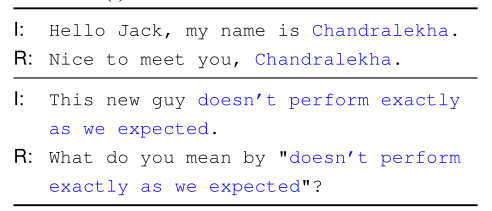
\includegraphics[width=9cm,height=3cm]{pictures/lr.jpg}
  \caption{the human language communication.For example, in the
  following two dialogue turns we observe differ-
  ent patterns in which some subsequences (colored
  blue) in the response (R) are copied from the input
  utterance (I)}
\end{figure}
    \item Both the canonical encoder-decoder and its
    variants with attention mechanism rely heavily
    on the representation of “meaning”, which \textcolor{red}{might
    not be sufficiently inaccurate in cases in which
    the system needs to refer to sub-sequences of in-
    put like entity names or dates}.
    \item In contrast, the copying mechanism is closer to the rote memorization in language processing of human being,
    deserving a different modeling strategy in neural
    network-based models. 
    \item We argue that it will benefit many Seq2Seq tasks to have an elegant unified
    model that can accommodate both understanding
    and rote memorization. Towards this goal, we pro-
    pose COPYNET,\textcolor{red}{ which is not only capable of the
    regular generation of words but also the operation
    of copying appropriate segments of the input sequence}. Despite the seemingly “hard” operation
    of copying, COPYNET can be trained in an end-to-
    end fashion. Our empirical study on both synthetic
    datasets and real world datasets demonstrates the
    efficacy of COPYNET.
    \end{itemize}

    \section{Background: Neural Models for
    Sequence-to-sequence Learning}
    Seq2Seq Learning can be expressed in a probabilistic view as maximizing the likelihood (or
    some other evaluation metrics (Shen et al., 2015))
    of observing the output (target) sequence given an
    input (source) sequence.

    \subsection{RNN Encoder-Decoder}

    RNN-based Encoder-Decoder is successfully applied to real world Seq2Seq tasks, first by Cho et
    al. (2014) and Sutskever et al. (2014), and then
    by (Vinyals and Le, 2015; Vinyals et al., 2015a).
    In the Encoder-Decoder framework, the source sequence $X = [x_1, ..., x_{TS}]$ is converted into a fixed
    length vector $c$ by the encoder RNN, i.e.

    $ h_t =f(x_t,h_{t-1});c=\phi({h_1,h_2,...h_{TS}})$


    where ${h_t}$ are the RNN states, c is the so-called
    context vector, $f$ is the dynamics function, and $\phi$
    summarizes the hidden states, e.g. choosing the
    last state $h_{TS}$. In practice it is found that gated
    RNN alternatives such as LSTM (Hochreiter and
    Schmidhuber, 1997) or GRU (Cho et al., 2014) of-
    ten perform much better than vanilla ones.
    The decoder RNN is to unfold the context vector c into the target sequence, through the following dynamics and prediction model:
    
    $ s_t=f(y_{t-1},s_{t-1},c) $


    $ p(y_t|y_{<t},X)=g( y_{t-1}, s_t,c) $     


    where $s_t$ is the RNN state at time $t$, $y_t$ is the predicted target symbol at $t$ (through function $g(·)$)
    with $y_{<t}$ denoting the history ${y_1, ..., y_{t−1}}$. The prediction model is typically a classifier over the
    vocabulary with, say, 30,000 words.

    \subsection{The Attention Mechanism}
    \textcolor{red}{The attention mechanism was first introduced to Seq2Seq (Bahdanau et al., 2014) to release the
    burden of summarizing the entire source into a
    fixed-length vector as context}. Instead, the attention uses a dynamically changing context $c_t$ in the
    decoding process. A natural option (or rather “soft
    attention”) is to represent $c_t$ as the weighted sum
    of the source hidden states, i.e.

    $c_t=\sum_{\tau =1}^{T_s}  \alpha_{t \tau}h_\tau;$


    $\alpha_{t \tau}= \frac{e^{\eta(s_{t-1},h_\tau)}}{\sum_{\tau'}e^{ \eta(s_{t-1},h_\tau') } } $

    where $\eta$ is the function that shows the correspondence strength for attention, approximated usually
    with a multi-layer neural network (DNN). Note that in (Bahdanau et al., 2014) the source sentence is 
    encoded with a Bi-directional RNN, making each hidden state $h_\tau$ aware of the contextual
    information from both ends.

    \section{COPYNET}
    From a cognitive perspective, the copying mechanism is related to rote memorization, requiring
    less understanding but ensuring high literal fidelity. From a modeling perspective, the copying
    operations are more rigid and symbolic, making
    it more difficult than soft attention mechanism to
    integrate into a fully differentiable neural model.
    In this section, we present COPYNET, a differentiable Seq2Seq model with “copying mechanism”,
    which can be trained in an end-to-end fashion with
    just gradient descent.
    \subsection{Model Overview}
    As illustrated in Figure 1, COPYNET is still an
    encoder-decoder (in a slightly generalized sense).
    The source sequence is transformed by Encoder
    into representation, which is then read by Decoder
    to generate the target sequence.

\begin{figure}[htbp]
    \centering
    \vspace{-0.35cm} 
    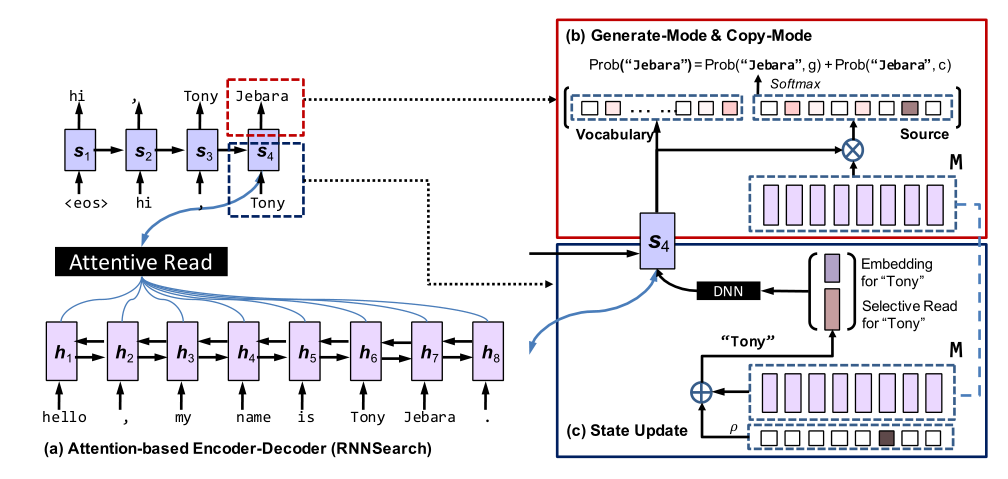
\includegraphics[width=14cm,height=8cm]{pictures/model.jpg}
    \caption{The overall diagram of COPYNET. For simplicity, we omit some links for prediction (see
    Sections 3.2 for more details).}
\end{figure}

    Encoder: Same as in (Bahdanau et al., 2014), a
    bi-directional RNN is used to transform the source
    sequence into a series of hidden states with equal
    length, with each hidden state ht corresponding to
    word $x_t$. This new representation of the source,
    ${h1, ..., h_{T_S}}$, is considered to be a short-term
    memory (referred to as M in the remainder of the
    paper), which will later be accessed in multiple
    ways in generating the target sequence (decoding).

    Decoder: An RNN that reads M and predicts
    the target sequence. It is similar with the canoni-
    cal RNN-decoder in (Bahdanau et al., 2014), with
    however the following important differences.

    • Prediction: COPYNET predicts words based
    on a mixed probabilistic model of two modes,
    namely the generate-mode and the copy-
    mode, where the latter picks words from the
    source sequence (see Section 3.2);

    • State Update: the predicted word at time $t−1$
    is used in updating the state at t, but COPY-
    NET uses not only its word-embedding but
    also its corresponding location-specific hid-
    den state in M (if any) (see Section 3.3 for
    more details);

    • Reading M: in addition to the attentive read
    to M, COPYNET also has“selective read”
    to M, which leads to a powerful hybrid of
    content-based addressing and location-based
    addressing (see both Sections 3.3 and 3.4 for
    more discussion).


    \subsection{Prediction with Copying and Generation}
    \textcolor{red}{We assume a vocabulary V = {v1, ..., vN}, and use UNK for any out-of-vocabulary (OOV) word.
    In addition, we have another set of words $\chi$ , for
    all the unique words in source sequence $X =
    {x1, ..., xTS}$. Since $\chi$ may contain words not
    in V, copying sub-sequence in X enables COPY-
    NET to output some OOV words. In a nutshell,
    the instance-specific vocabulary for source X is
    $V \cup UNK \cup  \chi $ }.

    Given the decoder RNN state st at time t to-
    gether with M, the probability of generating any
    target word $y_t$, is given by the “mixture” of proba-
    bilities as follows

    $   p(y_t| s_t,y_{t-1},c_t,M)=p(y_t,g|s_t,y_{t-1},c_t,M)+p(y_t,c|s_t,y_{t-1},c_t,M)                       $

    where g stands for the generate-mode, and c the
    copy mode. The probability of the two modes are
    given respectively by


    $   p(y_t,g|.)=\left\{
        \begin{matrix}
        \frac{1}{Z}e^{ \psi_g (y_t)}& y_t \in  V\\
        0 & y_t \in \chi \cap \bar{V}\\
        \frac{1}{Z}e^{ \psi_g (UNK)} & y_t \not \in V \cup \chi
        \end{matrix}
        \right.                                   $

        $  p(y_t,c|.)=\left\{
            \begin{matrix}
            \frac{1}{Z}\sum{j:x_j=y_t}e^{ \psi_c (x_j)}& y_t \in  V\\
            0 & otherwise
            \end{matrix}
            \right.                                   $
    
    where $\psi_g(·)$ and $\psi c(·)$ are score functions for
    generate-mode and copy-mode, respectively, and
    Z is the normalization term shared by the two
    modes, $Z = \sum{v \in V \cup {UNK}} e^{\psi_g(v)}  +\sum_{x \in X} e^{\psi_c(x)} $.
    Due to the shared normalization term, the two
    modes are basically competing through a softmax
    function (see Figure 1 for an illustration with example), rendering Eq.(4) deviated from the canonical definition of mixture model (McLachlan and
    Basford, 1988). This is also pictorially illustrated
    in Figure 2. The score of each mode is calculated:
    al., 2014) is used, i.e.

    \begin{figure}[htbp]
        \centering
        \vspace{-0.35cm} 
        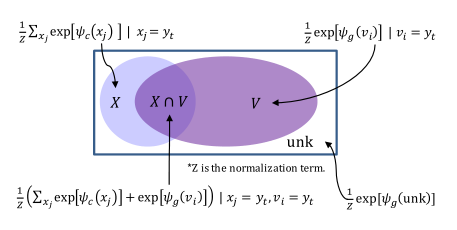
\includegraphics[width=14cm,height=8cm]{pictures/x.jpg}
        \caption{The illustration of the decoding probability $p(y_t|·)$ as a 4-class classifier.}
    \end{figure}

    Generate-Mode: The same scoring function as
    in the generic RNN encoder-decoder (Bahdanau et al., 2014) is used, i.e.
    
    $\psi_g(y_t = v_i) = {v_i}^T  W_o s_t, v_i \in  V \cup UNK $
    
    ,where $ W_o \in R^{(N+1)×d_s} $ and $v_i$  is the one-hot in dicator vector for $v_i$.

    Copy-Mode: The score for “copying” the word $x_j$ is calculated as
    $  \psi_c(y_t = x_j) = \sigma({h_j}^TW_c)s_t,x_j \in \chi    $

    where $W_c \in R^{d_h}×d_s$, and $\sigma$ is an activation
    that is either an identity or a non-linear function
    such as tanh. When calculating the copy-mode
    score, we use the hidden states ${h_1, ..., h_{T_S}}$ to
    “represent” each of the word in the source se-
    quence ${x_1, ..., x_{T_S}}$ since the bi-directional RNN
    encodes not only the content, but also the location
    information into the hidden states in M. The loca-
    tion informaton is important for copying (see Sec-
    tion 3.4 for related discussion). Note that we sum
    the probabilities of all $x_j$ equal to $y_t$ in Eq. (6) con-
    sidering that there may be multiple source symbols
    for decoding $y_t$. Naturally we let $p(y_t, c|·) = 0 $ if
    $y_t$ does not appear in the source sequence, and set
    $p(y_t, g|·) = 0$ when $y_t$ only appears in the source.


    \subsection{State Update}

    COPYNET updates each decoding state $s_t$ with
    the previous state $s_{t−1}$, the previous symbol $y_{t−1}$
    and the context vector $c_t$ following Eq. (2) for the
    generic attention-based Seq2Seq model. However,
    there is some minor changes in the $y_{t−1}→s_t$ path
    for the copying mechanism. More specifically,
    $y_{t−1}$ will be represented as $[e(y_{t−1}); \zeta (y_{t−1})]^T$,
    where $e(y_{t−1})$ is the word embedding associated
    with $y_{t−1}$, while $\zeta(y_t−1)$ is the weighted sum of
    hidden states in M corresponding to $y_t$.

    $ \zeta(y_{t-1})=\sum_{\tau =1}^{T_s}\rho_{t\tau}h_\tau$
    
    $  \rho_{t\tau}=\left\{
        \begin{matrix}
        \frac{1}{K}p(x_\tau,c|s_{t-1},M) & x_\tau = y_{t-1}\\
        0 & otherwise
        \end{matrix}
        \right.                                   $



    where K is the normalization term which equals
    $\sum_{\tau':x_{\tau'}=y_{t-1}}{p(x_{\tau'},c|s_{t-1},M)}$, considering there
    may exist multiple positions with $y_{t−1}$ in the
    source sequence. In practice, $\rho_{t \tau} $ is often con-
    centrated on one location among multiple appear-
    ances, indicating the prediction is closely bounded
    to the location of words.

    In a sense $\zeta(y_{t−1})$ performs a type of read to
    M similar to the attentive read (resulting $c_t$) with
    however higher precision. In the remainder of
    this paper, $\zeta(y_{t−1})$ will be referred to as selective
    read.  $\zeta(y_{t−1})$ is specifically designed for the copy
    mode: with its pinpointing precision to the cor-
    responding $y_{t−1}$, it naturally bears the location of
    $y_{t−1}$ in the source sequence encoded in the hidden
    state. As will be discussed more in Section 3.4,
    this particular design potentially helps copy-mode
    in covering a consecutive sub-sequence of words.
    If $y_{t−1}$ is not in the source, we let $\zeta(y_{t−1})=0$.


    \subsection{Hybrid Addressing of M}
    We hypothesize that COPYNET uses a hybrid
    strategy for fetching the content in M, which com-
    bines both content-based and location-based ad-
    dressing. Both addressing strategies are coordi-
    nated by the decoder RNN in managing the atten-
    tive read and selective read, as well as determining
    when to enter/quit the copy-mode.
    Both the semantics of a word and its location
    in X will be encoded into the hidden states in M
    by a properly trained encoder RNN. Judging from
    our experiments, the attentive read of COPYNET is
    driven more by the semantics and language model,
    therefore capable of traveling more freely on M,
    even across a long distance. On the other hand,
    once COPYNET enters the copy-mode, the selec-
    tive read of M is often guided by the location in-
    formation. As the result, the selective read often
    takes rigid move and tends to cover consecutive
    words, including UNKs. Unlike the explicit de-
    sign for hybrid addressing in Neural Turing Ma-
    chine (Graves et al., 2014; Kurach et al., 2015),
    COPYNET is more subtle: it provides the archi-
    tecture that can facilitate some particular location-
    based addressing and lets the model figure out the
    details from the training data for specific tasks.


    Location-based Addressing: With the location
information in $\{h_i\}$, the information flow
 $\zeta(y_{t−1}) update → s_t  predict → y_t sel.read→ \zeta (y_t)$
provides a simple way of “moving one step to the
right” on X. More specifically, assuming the selective read 
$\zeta{y_{t−1}}$ concentrates on the $l^th$ word
in X, the state-update operation $ \zeta(y_{t−1}) update →s_t$
acts as “location ← location+1”, making st
favor the $(l+1)^th$ word in X in the prediction
$s_t predict → y_t $ in copy-mode. This again leads to
the selective read $\hat{h}_t sel. read →\zeta(y_t)$ for the state up-
date of the next round.
Handling Out-of-Vocabulary Words :Although
it is hard to verify the exact addressing strategy as
above directly, there is strong evidence from our
empirical study. Most saliently, a properly trained
COPYNET can copy a fairly long segment full of
OOV words, despite the lack of semantic infor-
mation in its M representation. This provides a
natural way to extend the effective vocabulary to
include all the words in the source. Although this
change is small, it seems quite significant empiri-
cally in alleviating the OOV problem. Indeed, for
many NLP applications (e.g., text summarization
or spoken dialogue system), much of the OOV
words on the target side, for example the proper
nouns, are essentially the replicates of those on the
source side.

    \section{Learning}
    Although the copying mechanism uses the “hard”
    operation to copy from the source and choose to
    paste them or generate symbols from the vocabulary, COPYNET is fully differentiable and can
    be optimized in an end-to-end fashion using back-
    propagation. Given the batches of the source and
    target sequence $\{X\}_N$ and $\{Y\}_N$, the objectives
    are to minimize the negative log-likelihood:

    $    L=-\frac{1}{N}\sum_{k=1}^{N}\sum_{t=1}^{T}log[p({y_t}^k|{y_{<t}}^k,X_k)]                             $


    where we use superscript to index the instances.
    Since the tribalistic model for observing any target word is a mixture of generate-mode and copy-
    mode, there is no need for any additional labels
    for modes. The network can learn to coordinate
    the two modes from data. More specifically, if one
    particular word ${y_t}^k$ can be found in the source sequence, the copy-mode will contribute to the mixture model, and the gradient will more or less en-
    courage the copy-mode; otherwise, the copy-mode
    is discouraged due to the competition from the
    shared normalization term Z. In practice, in most
    cases one mode dominates.


    \section{Experiments}
    We report our empirical study of COPYNET on the
    following three tasks with different characteristics
    1. A synthetic dataset on with simple patterns;
    2. A real-world task on text summarization;
    3. A data set for simple single-turn dialogues.
    \subsection{Synthetic Dataset}
    Dataset: We first randomly generate transforma-
    tion rules with 5-20 symbols and variables x \&
    y, e.g.

     $a b x c d y e f → g h x m,$

    with {a b c d e f g h m} being regular symbols
    from a vocabulary of size 1,000. As shown in the
    table below, each rule can further produce a num-
    ber of instances by replacing the variables with
    randomly generated subsequences (1-15 sym-
    bols) from the same vocabulary. We create five
    types of rules, including “x → ∅”. The task is
    to learn to do the Seq2Seq transformation from
    the training instances. This dataset is designed to
    study the behavior of COPYNET on handling simple and rigid patterns. Since the string to repeat
    are random, they can also be viewed as some extreme cases of rote memorization.
    

    Experimental Setting: We select 200 artificial
    rules from the dataset, and for each rule 200 in-
    stances are generated, which will be split into
    training (50%) and testing (50%). We compare
    the accuracy of COPYNET and the RNN Encoder-
    Decoder with (i.e. RNNsearch) or without attention (denoted as Enc-Dec). For a fair comparison, we use bi-directional GRU for encoder and
    another GRU for decoder for all Seq2Seq models,
    with hidden layer size = 300 and word embedding
    dimension = 150. We use bin size = 10 in beam
    search for testing. The prediction is considered
    correct only when the generated sequence is ex-
    actly the same as the given one.


    \begin{figure}[htbp]
        \centering
        \vspace{-0.35cm} 
        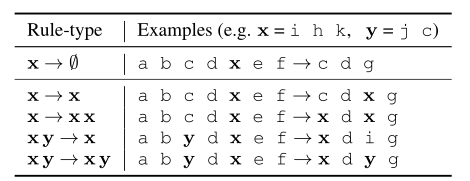
\includegraphics[width=14cm,height=8cm]{pictures/zc.jpg}
        \caption{ data }
    \end{figure}

    It is clear from Table 1 that COPYNET signifi-
    cantly outperforms the other two on all rule-types
    except “x → ∅”, indicating that COPYNET can ef-
    fectively learn the patterns with variables and ac-
    curately replicate rather long subsequence of sym-
    bols at the proper places.This is hard to Enc-Dec
    due to the difficulty of representing a long se-
    quence with very high fidelity. This difficulty can
    be alleviated with the attention mechanism. How-
    ever attention alone seems inadequate for handling
    the case where strict replication is needed.

    A closer look (see Figure 3 for example) reveals that the decoder is dominated by copy-mode
    when moving into the subsequence to replicate,
    and switch to generate-mode after leaving this
    area, showing COPYNET can achieve a rather precise coordination of the two modes.
    

    \begin{figure}[htbp]
        \centering
        \vspace{-0.35cm} 
        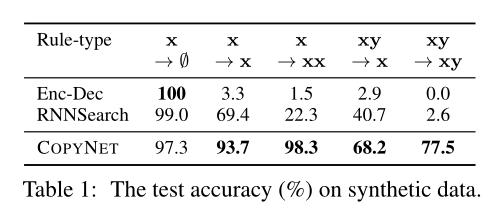
\includegraphics[width=14cm,height=8cm]{pictures/jg.jpg}
        \caption{ result }
    \end{figure}



    \subsection{Text Summarization}

    Automatic text summarization aims to find a condensed representation which can capture the core
    meaning of the original document. It has been
    recently formulated as a Seq2Seq learning problem in (Rush et al., 2015; Hu et al., 2015), which
    essentially gives abstractive summarization since
    the summary is generated based on a representation of the document. In contrast, extractive
    summarization extracts sentences or phrases from
    the original text to fuse them into the summaries,
    therefore making better use of the overall structure of the original document. In a sense, COPY-
    NET for summarization lies somewhere between
    two categories, since part of output summary is actually extracted from the document (via the copying mechanism), which are fused together possibly with the words from the generate-mode.

    Dataset: We evaluate our model on the recently
    published LCSTS dataset (Hu et al., 2015), a large
    scale dataset for short text summarization. The
    dataset is collected from the news medias on Sina
    Weibo1 including pairs of (short news, summary)
    in Chinese. Shown in Table 2, PART II and III are
    manually rated for their quality from 1 to 5. Following the setting of (Hu et al., 2015) we use Part I as the training set and and the subset of Part III
    scored from 3 to 5 as testing set.
    
    \begin{figure}[htbp]
        \centering
        \vspace{-0.35cm} 
        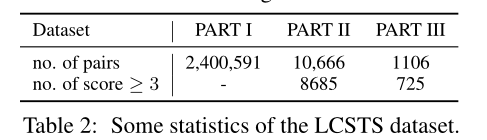
\includegraphics[width=14cm,height=8cm]{pictures/data.jpg}
        \caption{ TS data }
    \end{figure}


    Experimental Setting: We try COPYNET that is
based on character (+C) and word (+W). For the
word-based variant the word-segmentation is ob-
tained with jieba2. We set the vocabulary size to
3,000 (+C) and 10,000 (+W) respectively, which
are much smaller than those for models in (Hu
et al., 2015). For both variants we set the em-
bedding dimension to 350 and the size of hidden
layers to 500. Following (Hu et al., 2015), we
evaluate the test performance with the commonly
used ROUGE-1, ROUGE-2 and ROUGE-L (Lin,
2004), and compare it against the two models in
(Hu et al., 2015), which are essentially canonical
Encoder-Decoder and its variant with attention.

It is clear from Table 3 that COPYNET beats
the competitor models with big margin. Hu
et al. (2015) reports that the performance of a
word-based model is inferior to a character-based
one. One possible explanation is that a word-
based model, even with a much larger vocabulary
(50,000 words in Hu et al. (2015)), still has a large
proportion of OOVs due to the large number of en-
tity names in the summary data and the mistakes
in word segmentation. COPYNET, with its ability
to handle the OOV words with the copying mech-
anism, performs however slightly better with the
word-based variant.

\begin{figure}[htbp]
    \centering
    \vspace{-0.35cm} 
    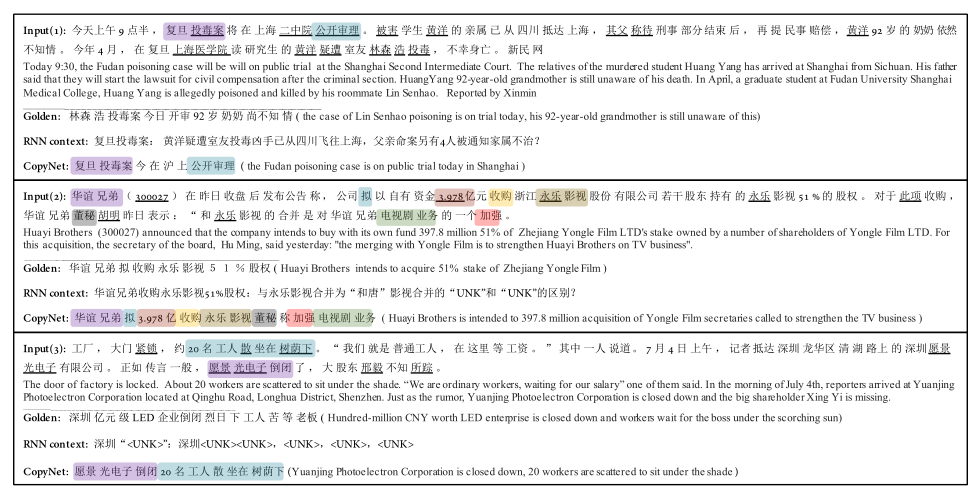
\includegraphics[width=15cm,height=9cm]{pictures/TS.jpg}
    \caption{ Examples of COPYNET on LCSTS compared with RNN context. Word segmentation is
    applied on the input, where underlined are OOV words. The highlighted words (with different colors)
    are those words with copy-mode probability higher than the generate-mode. We also provide literal
    English translation for the document, the golden, and COPYNET, while omitting that for RNN context
    since the language is broken. }
\end{figure}

We make the following interesting observations
about the summary from textscCopyNet (Figure 4,
and more in the supplementary material): 1) most
words are from copy-mode, but the summary is
usually still fluent; 2) COPYNET tends to cover
consecutive words in the original document, but it
often puts together segments far away from each
other, indicating a sophisticated coordination of
content-based addressing and location-based ad-
dressing; 3) COPYNET handles OOV words really
well: it can generate acceptable summary for doc-
ument with many OOVs, and even the summary
itself often contains many OOV words. In con-
trast, the canonical RNN-based approaches often
fail in cases like that.
It is quite intriguing that COPYNET can often
find important parts of the document, a behav-
ior with the characteristics of extractive summa-
rization, while it often generate words to “con-
nect” those words, showing its aspect of abstrac-
tive summarization

 
    \subsection{Single-turn Dialogue}


    \begin{figure}[htbp]
        \centering
        \vspace{-0.35cm} 
        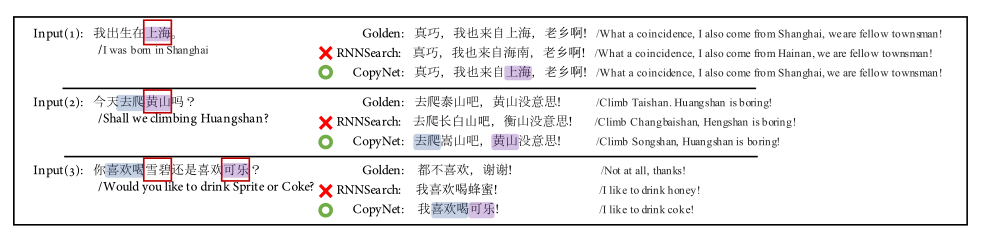
\includegraphics[width=13cm,height=6cm]{pictures/dh.jpg}
        \caption{ Examples on the testing set of DS-II shown as the input text and golden, with the outputs
        of RNNSearch and CopyNet. Words in red rectangles are unseen in the training set. The highlighted
        words (with different colors) are those words with copy-mode probability higher than the generate-mode.
        Green cirles (meaning correct) and red cross (meaning incorrect) are given based on human judgment on
        whether the response is appropriate. }
    \end{figure}


    \section{Related Work}
    \begin{itemize}
    \item \textcolor{red}{Our work is partially inspired by the recent work
    of Pointer Networks (Vinyals et al., 2015a), in
    which a pointer mechanism (quite similar with the
    proposed copying mechanism) is used to predict
    the output sequence directly from the input. In ad-
    dition to the difference with ours in application,
    (Vinyals et al., 2015a) cannot predict outside of
    the set of input sequence, while COPYNET can
    naturally combine generating and copying.}
    \item \textcolor{red}{COPYNET is also related to the effort to solve
    the OOV problem in neural machine translation.
    Luong et al. (2015) introduced a heuristics to post-
    process the translated sentence using annotations
    on the source sentence. In contrast COPYNET addresses the OOV problem in a more systemic way
    with an end-to-end model. However, as COPYNET copies the exact source words as the output, it
    cannot be directly applied to machine translation.}
    \item \textcolor{red}{The copying mechanism can also be viewed as
    carrying information over to the next stage without
    any nonlinear transformation. Similar ideas are
    proposed for training very deep neural networks in
    (Srivastava et al., 2015; He et al., 2015) for clas-
    sification tasks, where shortcuts are built between
    layers for the direct carrying of information.}

    \end{itemize}

    \section{Conclusion and Future Work}
    We proposed COPYNET to incorporate the copying mechanism into Seq2Seq learning framework.For future work, we will extend this idea to the task where the source and target are in different
    languages, for example, machine translation.

    \section{Personal understanding}
    \subsection{Paper structure}

    \begin{figure}[htbp]
        \centering
        \vspace{-0.35cm} 
        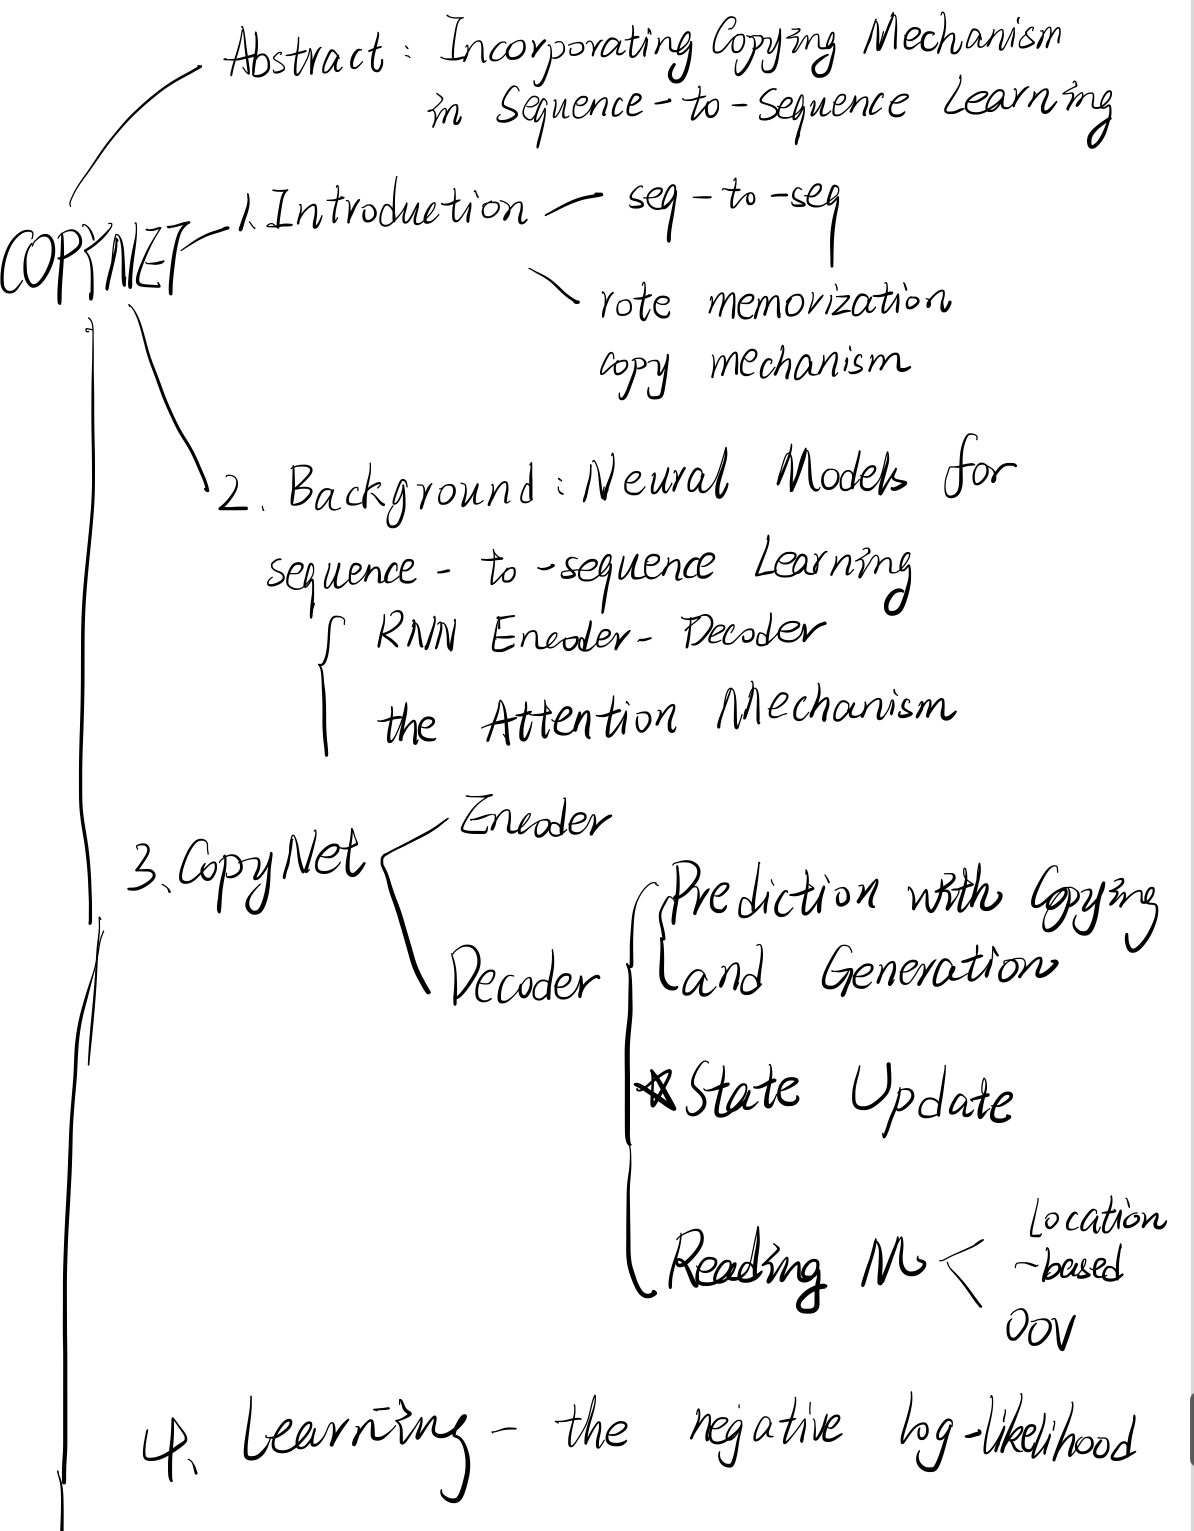
\includegraphics[width=14cm,height=18cm]{pictures/a1.jpg}
        \caption{Paper: COPYNET.}
    \end{figure}


    \begin{figure}[htbp]
        \centering
        \vspace{-0.35cm} 
        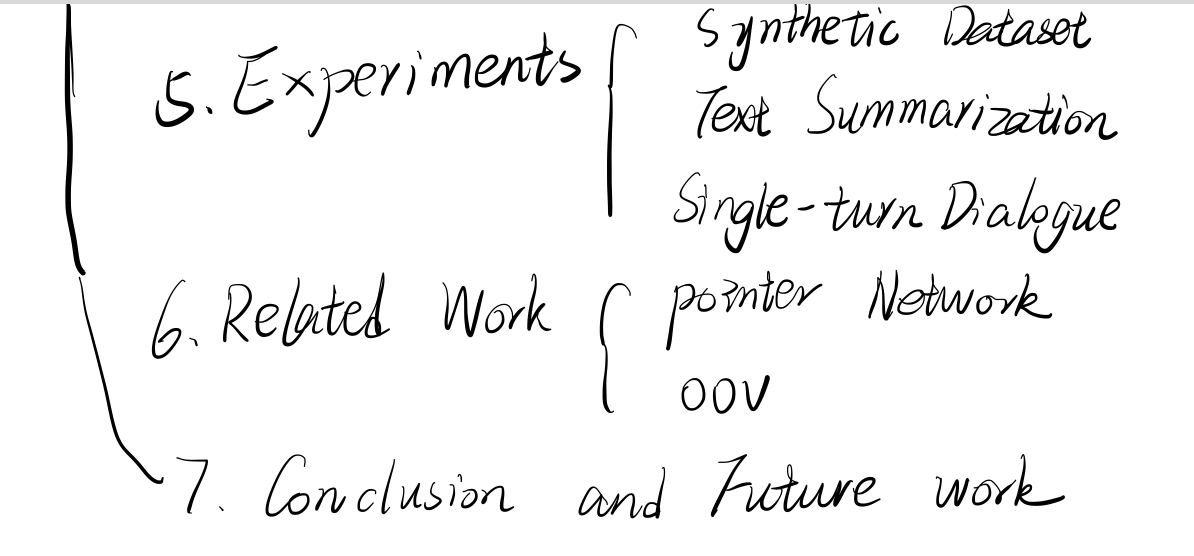
\includegraphics[width=14cm,height=8cm]{pictures/a2.jpg}
        \caption{Paper: COPYNET..}
    \end{figure}



    \subsection{The problem to solve}
    \begin{itemize}
    \item the rote memorization; copying mechanism

    \begin{figure}[htbp]
        \centering
        %\vspace{-0.35cm} 
        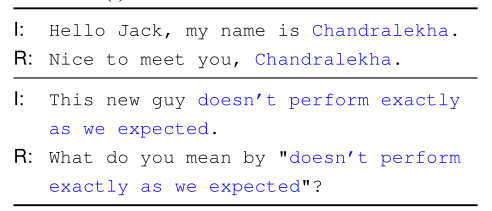
\includegraphics[width=9cm,height=3cm]{pictures/lr.jpg}
        \caption{the human language communication.For example, in the
        following two dialogue turns we observe differ-
        ent patterns in which some subsequences (colored
        blue) in the response (R) are copied from the input
        utterance (I)}
      \end{figure}


    \item out-of-vocabulary (OOV) 
    \end{itemize}


    \subsection{The innovation work}

    \begin{figure}[htbp]
        \centering
        \vspace{-0.35cm} 
        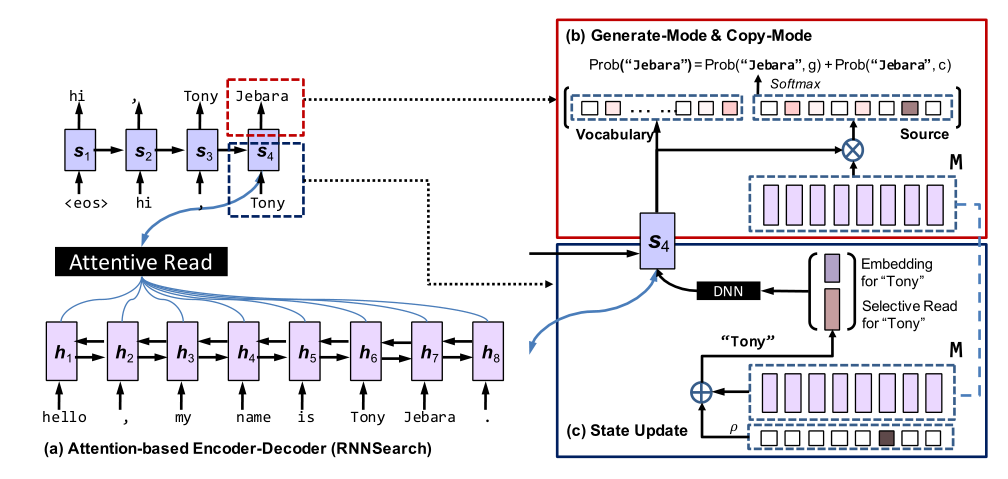
\includegraphics[width=14cm,height=8cm]{pictures/model.jpg}
        \caption{The overall diagram of COPYNET.}
    \end{figure}


        \begin{figure}[htbp]
            \centering
            \vspace{-0.35cm} 
            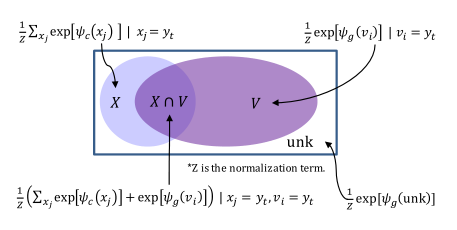
\includegraphics[width=14cm,height=8cm]{pictures/x.jpg}
            \caption{The illustration of the decoding probability $p(y_t|·)$ as a 4-class classifier.}
        \end{figure}


   
        
    \begin{figure}[htbp]
        \centering
        \vspace{-0.35cm} 
        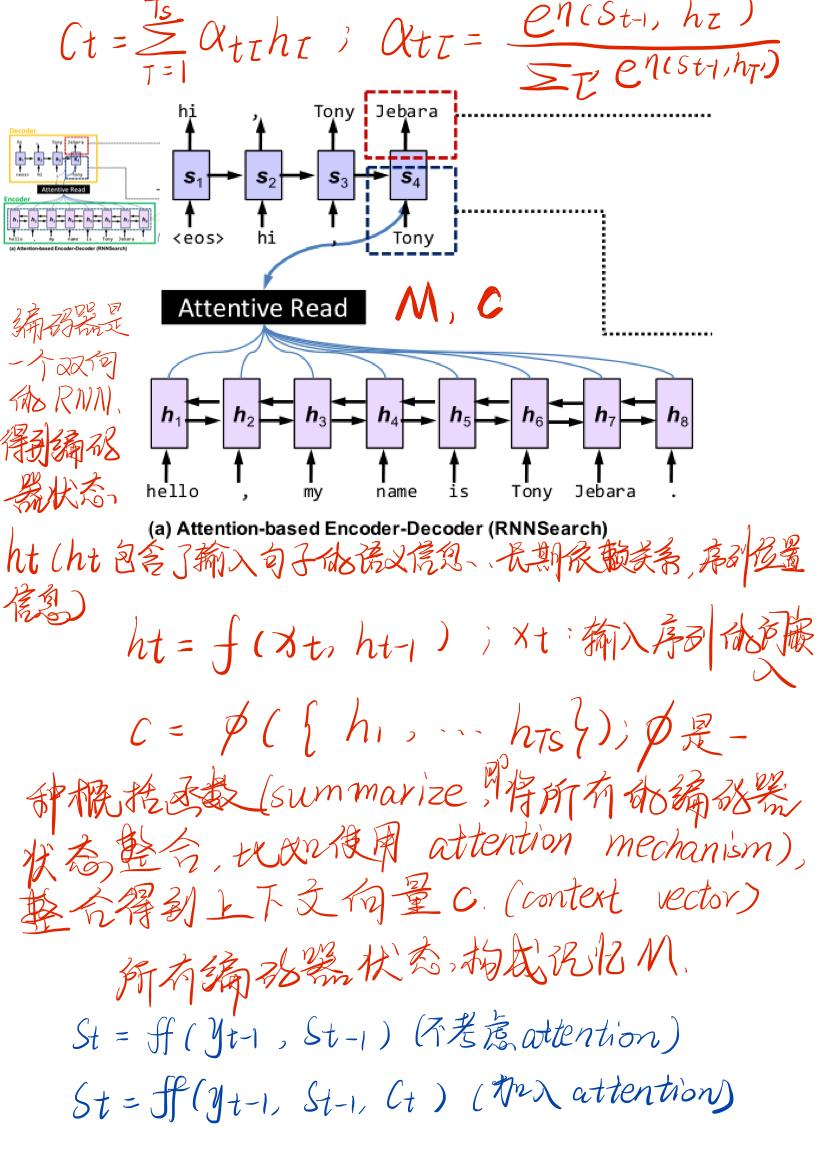
\includegraphics[width=13cm,height=18cm]{pictures/en.jpg}
        \caption{Attention-based Encoder-Decoder (RNNSearch)}
    \end{figure}

    \begin{figure}[htbp]
        \centering
        \vspace{-0.35cm} 
        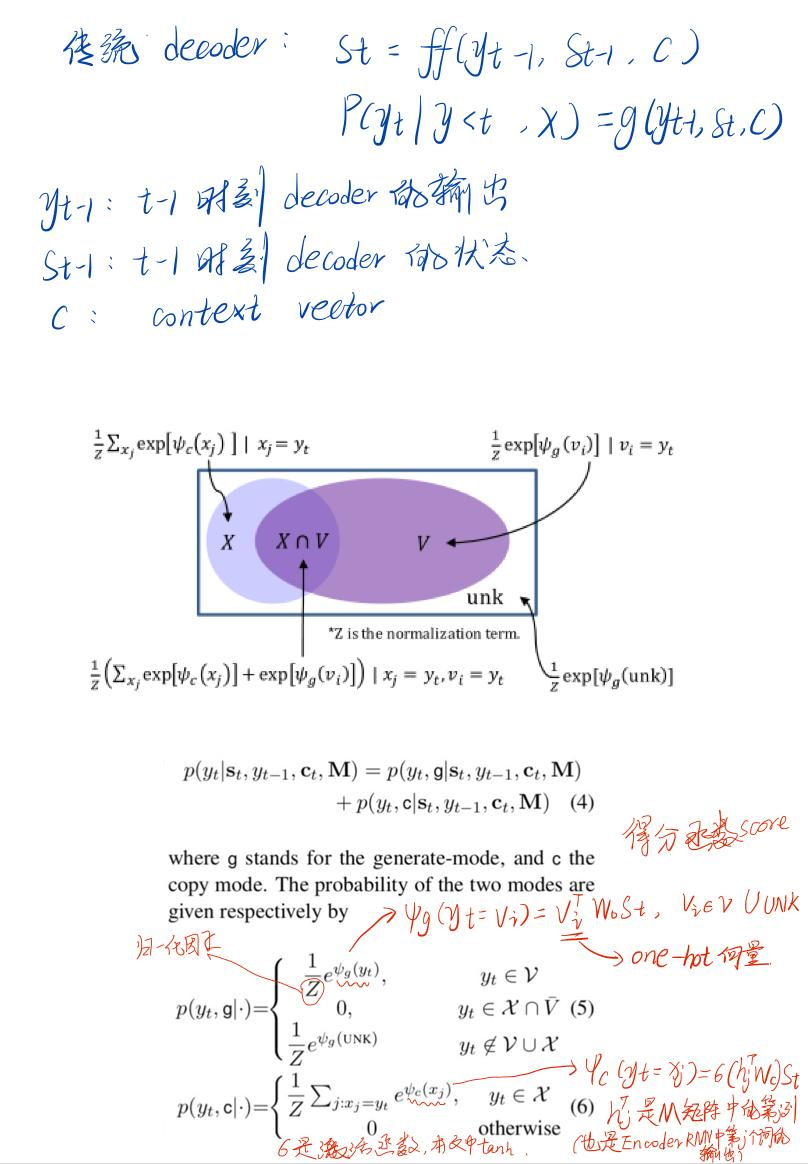
\includegraphics[width=14cm,height=18cm]{pictures/p.jpg}
        \caption{Prediction with Copying and Generation(Generate-Mode \& Copy-Mode)}
    \end{figure}

    \begin{figure}[htbp]
        \centering
        \vspace{-0.35cm} 
        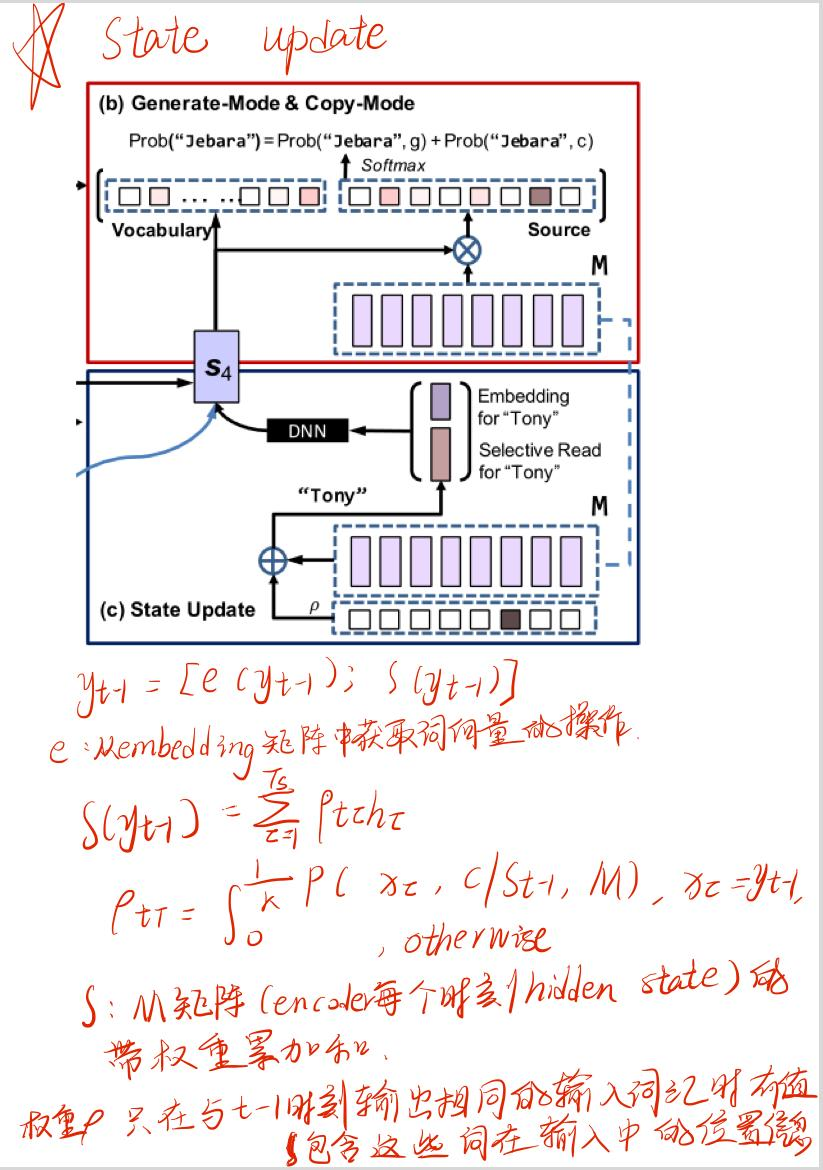
\includegraphics[width=14cm,height=18cm]{pictures/su.jpg}
        \caption{State update}
    \end{figure}

    \begin{figure}[htbp]
        \centering
        \vspace{-0.35cm} 
        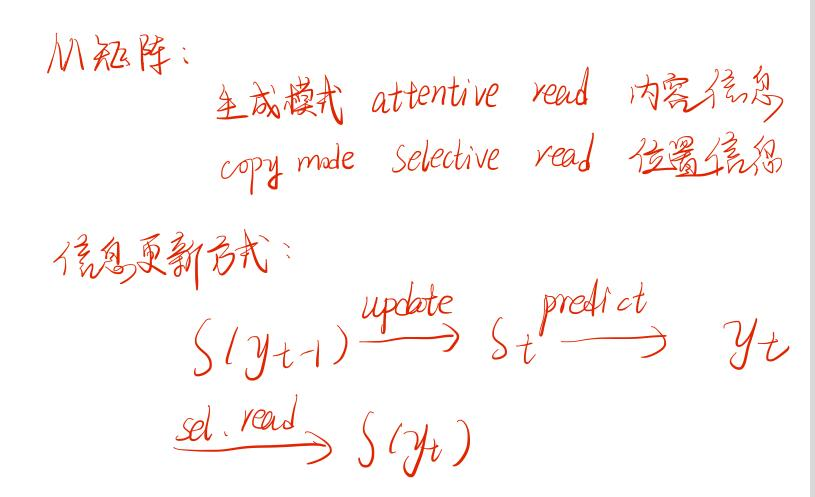
\includegraphics[width=14cm,height=8cm]{pictures/M.jpg}
        \caption{Hybrid Addressing of M}
    \end{figure}

  
    \subsection{The code analysis}



    \url{https://github.com/lspvic/CopyNet/blob/master/copynet.py}
   
    \url{https://github.com/adamklec/copynet/blob/master/model/copynet_decoder.py}   
    
    \url{https://github.com/mjc92/CopyNet/blob/master/models/copynet.py}

    \url{https://github.com/YinpeiDai/Seq2Seq-Models/blob/master/model.py}

    \url{https://github.com/MultiPath/CopyNet/tree/master/emolga/models}




    \end{document}

